\documentclass[notitlepage,aps,prd,nofootinbib]{revtex4-1}

\usepackage{subfig}
%\usepackage[colorinlistoftodos]{todonotes}
\usepackage{float}

%\usepackage[protrusion=true,expansion=true]{microtype}
\usepackage{amsmath}
\usepackage{amssymb}
\usepackage{bbm}
\usepackage{ulem}
%\usepackage{feynmp-auto}
%\usepackage{slashed}
%\usepackage[absolute,overlay]{textpos}
\usepackage[usenames, dvipsnames]{color}
\usepackage{graphicx}
\usepackage{listings}
\usepackage{epsfig}
\usepackage{hyperref}
%\usepackage{tikz}
\usepackage{enumerate}
%\usepackage{fixltx2e} % buggy
\usepackage[compatibility=false]{caption}
%\usepackage{subcaption} % doesn't work with subfigure
\usepackage{pdfpages}
%\usepackage{setspace}
\usepackage{verbatim}

% Turn off meaningless float warnings
\usepackage{silence}
\WarningFilter{revtex4-1}{Repair the float}

\DeclareRobustCommand{\orderof}{\ensuremath{\mathcal{O}}}

\definecolor{dukeblue}{RGB}{0,0,156}
\definecolor{dukedarkblue}{RGB}{0,26,87}
\definecolor{dukeblack}{RGB}{79,79,79}
\definecolor{dukegray}{RGB}{79,79,79}
\definecolor{dukesecbrown}{RGB}{217,200,158}
\definecolor{dukesecblue}{RGB}{127,169,174}

%\renewcommand*{\thefootnote}{\fnsymbol{footnote}}

%%%%%%%%%%%%%%%%%%%%%%%%%%%%%%%%%%%%%%%%%%%%%%%%%%%%%%%%%%%%%%%%%%%%%%%%%%%%%%%%%%%%%
\hypersetup{
    breaklinks,
    baseurl       = http://,
    pdfborder     = 0 0 0,
    pdfpagemode   = UseNone,% do not show thumbnails or bookmarks on opening
    pdfstartpage  = 1,
    bookmarksopen = true,
    bookmarksdepth= 2,% to show sections and subsections
% revtex needs author and title declared after \begin{document}, so have to hard code them...
%    pdfauthor     = {\@author},
%    pdftitle      = {\@title},
    pdfauthor     = {Matthew Epland},
    pdftitle      = {Phys 566 Midterm},
    pdfsubject    = {},
    pdfkeywords   = {}}


% Code import settings
%%%%%%%%%%%%%%%%%%%%%%%%%%%%%%%%%%%%%%%%%%%%%%%%%%%%%%%%%%%%%%%%%%%%%%%%%%%%%%%%%%%%%
\definecolor{mygreen}{rgb}{0,0.6,0}
\definecolor{mygray}{rgb}{0.5,0.5,0.5}
\definecolor{mymauve}{rgb}{0.58,0,0.82}

%\lstset{ %
\lstdefinestyle{python}{ %
  backgroundcolor=\color{white},   % choose the background color; you must add \usepackage{color} or \usepackage{xcolor}
  basicstyle=\scriptsize,          % the size of the fonts that are used for the code
  breakatwhitespace=false,         % sets if automatic breaks should only happen at whitespace
  breaklines=true,                 % sets automatic line breaking
  captionpos=b,                    % sets the caption-position to bottom
  commentstyle=\color{mygreen},    % comment style
  deletekeywords={...},            % if you want to delete keywords from the given language
  escapeinside={\%*}{*)},          % if you want to add LaTeX within your code
  extendedchars=true,              % lets you use non-ASCII characters; for 8-bits encodings only, does not work with UTF-8
  frame=single,	                   % adds a frame around the code
  keepspaces=true,                 % keeps spaces in text, useful for keeping indentation of code (possibly needs columns=flexible)
  keywordstyle=\color{blue},       % keyword style
  language=Python,                 % the language of the code
  otherkeywords={*,...},           % if you want to add more keywords to the set
  numbers=left,                    % where to put the line-numbers; possible values are (none, left, right)
  numbersep=5pt,                   % how far the line-numbers are from the code
  numberstyle=\tiny\color{mygray}, % the style that is used for the line-numbers
  rulecolor=\color{black},         % if not set, the frame-color may be changed on line-breaks within not-black text (e.g. comments (green here))
  showspaces=false,                % show spaces everywhere adding particular underscores; it overrides 'showstringspaces'
  showstringspaces=false,          % underline spaces within strings only
  showtabs=false,                  % show tabs within strings adding particular underscores
  stepnumber=5,                    % the step between two line-numbers. If it's 1, each line will be numbered
  stringstyle=\color{mymauve},     % string literal style
  tabsize=2,	                   % sets default tabsize to 2 spaces
%  title=\lstname                   % show the filename of files included with \lstinputlisting; also try caption instead of title
  title={\protect\filename@parse{\lstname}\protect\filename@base.\filename@ext},
  firstnumber=0,
%  linewidth=0.95\textwidth
  xleftmargin=0.01\textwidth,
  xrightmargin=0.01\textwidth
}

\lstdefinestyle{output}{ %
  backgroundcolor=\color{white},   % choose the background color; you must add \usepackage{color} or \usepackage{xcolor}
  basicstyle=\scriptsize,          % the size of the fonts that are used for the code
  breakatwhitespace=false,         % sets if automatic breaks should only happen at whitespace
  breaklines=true,                 % sets automatic line breaking
  captionpos=b,                    % sets the caption-position to bottom
  escapeinside={\%*}{*)},          % if you want to add LaTeX within your code
  frame=single,	                   % adds a frame around the code
  keepspaces=true,                 % keeps spaces in text, useful for keeping indentation of code (possibly needs columns=flexible)
  numbers=left,                    % where to put the line-numbers; possible values are (none, left, right)
  numbersep=5pt,                   % how far the line-numbers are from the code
  numberstyle=\tiny\color{mygray}, % the style that is used for the line-numbers
  rulecolor=\color{black},         % if not set, the frame-color may be changed on line-breaks within not-black text (e.g. comments (green here))
  stepnumber=5,                    % the step between two line-numbers. If it's 1, each line will be numbered
  tabsize=2,	                   % sets default tabsize to 2 spaces
%  title=\lstname                   % show the filename of files included with \lstinputlisting; also try caption instead of title
  title={\protect\filename@parse{\lstname}\protect\filename@base.\filename@ext},
  firstnumber=0,
%  linewidth=0.95\textwidth
  xleftmargin=0.01\textwidth,
  xrightmargin=0.01\textwidth
}

\newcommand{\degree}{\ensuremath{^{\circ}}}

% Select between raw and saved plots here
% \graphicspath{{../code/output/plots_for_paper/}}
\graphicspath{{../code/output/plots_for_paper_final/}}

%%%%%%%%%%%%%%%%%%%%%%%%%%%%%%%%%%%%%%%%%%%%%%%%%%%%%%%%%%%%%%%%%%%%%%%%%%%%%%%%%%%%%
\begin{document}

\title{PHYS 566 Midterm}
\author{Matthew Epland}
\affiliation{Department of Physics, Duke University, Durham, NC 27707, USA}

\date{\today}

\begin{abstract}
%No Time...
\end{abstract}\maketitle

\section{Introduction}
\label{sec:intro}
In this assignment the 2D electric potential of a dipole in a grounded circle was modeled computationally by solving the Poisson equation via the Jacobi and Simultaneous--Over--Relaxation methods. Reasonable agreement with the expected solution was observed, though the number of iterations did not scale for either method as expected. Additionally the magnetic field of a square current loop was found via numerically integrating the Biot--Savart Law with a Riemann sum. The result was compared to a similar circular current loop along the symmetry axis and found to be in excellent agreement. 

The Python source code used to produce these results can be found online at \url{http://github.com/mepland/PHYS_566_Computational_HW/tree/master/midterm/code}, and is included in Section~\ref{sec:code}.

\section{Theory}
\label{sec:theory}

\subsection{Numerical Solutions to the Poisson Equation}
\label{subsec:poisson_theory}
All of electrostatics can be described by a Poisson equation (\ref{eq:poisson}) with suitable boundary conditions, thus it is very important that we be able to solve such problems numerically. Once developed, a computational tool capable of solving (\ref{eq:poisson}) can produce potentials, $V\left(\mathbf{r}\right)$, for any charge distribution and boundary conditions fed into it.

\begin{equation} \label{eq:poisson}
\nabla^{2} V\left(\mathbf{r}\right) = -\frac{\rho\left(\mathbf{r}\right)}{\epsilon_{0}}
\end{equation}

In this assignment we will be using the Jacobi method and it's more complex extension, the Simultaneous--Over--Relaxation (SOR) method. To begin, we assume we are working in a 2D space\footnote{Extensions to higher dimensions can easily be written by altering the average over nearest--neighbors in the natural way.} with Cartesian coordinates quantized into squares of length $\Delta x$ and indexed by $\left(i,j\right)$. The Jacobi method can then be written formally as (\ref{eq:jacobi}), but is better understood as updating $V\left(i,j\right)$ for each square with the average of it's nearest--neighbors (NN), plus any source terms in the square\footnote{$\rho\left(i,j\right)\left(\Delta x\right)^{2} = Q\left(i,j\right)$}. Sweeps are made through the simulated region, updating each square in turn, until a convergence criteria is satisfied. Boundary conditions are included by holding $V\left(i,j\right) = V_{\mathrm{BC}}$ fixed at the appropriate $\left(i,j\right)$ points.

\begin{equation} \label{eq:jacobi}
V_{\mathrm{new}}\left(i,j\right)^{\mathrm{Jacobi}} = \frac{1}{2^2}\big( V_{\mathrm{old}}\left(i+1,j\right) + V_{\mathrm{old}}\left(i-1,j\right) +V_{\mathrm{old}}\left(i,j+1\right) +V_{\mathrm{old}}\left(i,j-1\right) \big) + \frac{1}{\epsilon_{0}} \rho\left(i,j\right)\left(\Delta x\right)^{2}
\end{equation}
While the Jacobi method is simple in form, it pays for this by being computationally expensive. If the simulated area itself is a square containing $L^{2} = n$ points, the Jacobi method will scale\footnote{One factor of $L^{2}$ comes from the method itself, the other from sweeping through all $L^{2}$ points.} as $\sim L^{2} \times L^{2} = n^{2}$. One immediate improvement on the Jacobi method is the Gauss--Seidel (GS) method (\ref{eq:GS}) that is exactly the same as the Jacobi method, but uses the last value of $V$ calculated, $V_{\mathrm{latest}}$, to compute the NN average instead of always relying on $V_{\mathrm{old}}$. This obviously saves memory, as only one array is needed to store the simulated region, but also improves the scaling behavior\footnote{$L^{2}$/2 from the method $\times$ $L^{2}$ from the sweeps.} to $\sim (1/2)n^{2}$.

\begin{equation} \label{eq:GS}
V_{\mathrm{new}}\left(i,j\right)^{\mathrm{GS}} = \frac{1}{2^2}\big( V_{\mathrm{latest}}\left(i+1,j\right) + V_{\mathrm{latest}}\left(i-1,j\right) +V_{\mathrm{latest}}\left(i,j+1\right) +V_{\mathrm{latest}}\left(i,j-1\right) \big) + \frac{1}{\epsilon_{0}} \rho\left(i,j\right)\left(\Delta x\right)^{2}
)
\end{equation}

The SOR method further improves on the GS method by taking the sweep--to-sweep change in $V\left(i,j\right)$ from the GS method (\ref{eq:SOR_DeltaV}), scaling it up by a factor of $\alpha$ and using the result as it's own sweep--to--sweep change (\ref{eq:SOR_V}). Without proof, the optimal value of $\alpha$ is given by (\ref{eq:SOR_alpha})\footnote{If $\alpha < 1$ SOR is worse than GS, if $\alpha = 1$ SOR reduces to GS, and if $\alpha \geq 2$ SOR becomes divergent.}. For $\alpha_{\mathrm{optimal}}$ the SOR method scales like $n^{3/2}$.

\begin{align}
\Delta V\left(i,j\right) &= V_{\mathrm{new}}\left(i,j\right)^{\mathrm{GS}} - V\left(i,j\right)_{\mathrm{old}} \label{eq:SOR_DeltaV} \\
V_{\mathrm{new}}\left(i,j\right)^{\mathrm{SOR}} &= \alpha \Delta V\left(i,j\right) + V\left(i,j\right)_{\mathrm{old}} \label{eq:SOR_V} \\
\alpha_{\mathrm{optimal}} &\approx \frac{2}{1+\pi/L} \label{eq:SOR_alpha} 
\end{align}

\subsection{Biot--Savart Law and Numerical Integration}
\label{subsec:biot_savart_theory}
Having dealt with electrostatics numerically we now turn to magnetostatics and the Biot--Savart Law (\ref{eq:biot_savart}). Here there is no need to solve equations, we simply need to integrate\footnote{Note that we could have also handled electrostatics in a similar manner by integrating Coulumb's law, but imposing boundary conditions could be quite troublesome. Magnetostatics problems usually don't have complex boundary conditions, so we can get away with the source integral method.} $\mathrm{d}\mathbf{B}\left(\mathbf{r}\right)$ over all current elements $I\,\mathrm{d}\mathbf{r}'$ to find $\mathbf{B}\left(\mathbf{r}\right)$.

\begin{equation} \label{eq:biot_savart}
\mathrm{d}\mathbf{B}\left(\mathbf{r}\right) = \frac{\mu_{0}I}{4\pi} \frac{\mathrm{d}\mathbf{r}' \times \left(\mathbf{r} - \mathbf{r}'\right)}{\left|\mathbf{r} - \mathbf{r}'\right|^{3}}
\end{equation}

There are a multitude of numerical integration schemes available, such as Simpson's rule and the trapezoid approximation. However for this assignment the simplest method, a midpoint Riemann sum (\ref{eq:riemann}), was sufficiently accurate\footnote{$\orderof\big(\left(\Delta x\right)^2\big)$} with reasonable computational requirements.

\begin{align} 
\int_{a}^{b} f\left(x\right)\,\mathrm{d}x &\approx \displaystyle\sum_{i=1}^{n} f\left(x_{i}^{*}\right) \Delta x \label{eq:riemann} \\
x_{i}^{*} &= a + \left(i-\frac{1}{2}\right) \Delta x \label{eq:reimann_midpoint}
\end{align}

The Riemann above is written in 1D, but is easily extended to 3D Cartesian coordinates as are needed to integrate $\mathrm{d}\mathbf{B}\left(\mathbf{r}\right)$. 


\clearpage
\section{Results}
\label{sec:results}

\subsection{Poisson Equation for a Dipole}
\label{subsec:poisson_results}
The electrostatics problem simulated in this assignment was that of a dipole inside a grounded circular boundary embedded in a 2D space. The dipole consisted of two point charges $Q/\epsilon_{0} = \pm1$ [Vm] separated by $a =$ 0.6 [m]. The coordinate system was chosen such that $\pm Q$ was located at $x = \pm a/2$, $y=0$. The circular boundary condition was simply $V\left(R\right) = 0$, $R =$ 10 [m].

The Jacobi and SOR methods as described in Section~\ref{subsec:poisson_theory} were used to simulate the problem on a grid of $L \times L$ squares with length $\Delta x$. Sweeps of the simulated area were run until the preset convergence criteria was satisfied. There were two possible convergence criteria, tolerance\footnote{Ideally a percentage tolerance would be used, but as $V\left(i,j\right)$ was frequently zero this would have caused divide by zero issues. These zero points could also not simply be ignored, or the simulation could end prematurely. One possible solution that I did not have time to implement and investigate, would be to divide by the nonzero option of $V_{\mathrm{new}}$ or $V_{\mathrm{old}}$. Even then $\epsilon$ would likely not converge, due to occasional very small denominators blowing up the sum. I saw this behavior firsthand when testing a na\"{\i}ve percent tolerance method.} $\epsilon$ (\ref{eq:epsilon_def}), and accuracy $A$ (\ref{eq:A_def}).

\begin{equation} \label{eq:epsilon_def} 
\epsilon_{\mathrm{sweep}} = \Bigg( \displaystyle\sum_{\forall (\mathrm{squares})} \left|V_{\mathrm{new}} - V_{\mathrm{old}}\right|\Bigg) / \Bigg( \displaystyle\sum_{\forall (\mathrm{squares})} 1 - \delta_{V_{\mathrm{new}},\,V_{\mathrm{old}}} \Bigg) < \epsilon
\end{equation}

\begin{equation} \label{eq:A_def} 
A_{\mathrm{sweep}} = \mathrm{maximum}|_{\forall (\mathrm{squares})} \bigg(\left|V_{\mathrm{new}} - V_{\mathrm{old}}\right|\bigg) < A
\end{equation}

See Figure~\ref{fig:part1a_V} for a $V\left(x, y\right)$ equapotential contour plot, and Figure~\ref{fig:part1a_Vr} for a plot of $V\left(r\right) = V\left(x,\,y=0\right)$ through the dipole's axis. In this case we can compare to the exact solution (\ref{eq:two_Qs}) and find that the simulation does a decent job except near the point charges themselves where the exact solution diverges to $\pm \infty$.

\begin{equation} \label{eq:two_Qs} 
V\left(r\right) = V\left(x,\,y=0\right) = \frac{Q}{4 \pi \epsilon_{0}} \bigg( \frac{1}{\left|r-a/2\right|} - \frac{1}{\left|r+a/2\right|} \bigg)
\end{equation}

\clearpage
\subsubsection{Part 1A}
\label{subsubsec:part_1a}

\begin{figure}[!htbc]
  \centering
  \includegraphics[width=.65\textwidth]{poisson_dipole/part_a/V_best_jacobi.pdf}
	{\par\nobreak\rule[9pt]{35em}{0.5pt}\vspace{-5mm}}
	\caption{$V\left(x, y\right)$, Jacobi method.}
	\label{fig:part1a_V}
\end{figure}

\begin{figure}[!htbc]
  \centering
  \includegraphics[width=.65\textwidth]{poisson_dipole/part_a/Vr_dipole_axis_best_jacobi.pdf}
	{\par\nobreak\rule[9pt]{35em}{0.5pt}\vspace{-5mm}}
	\caption{$V\left(r\right) = V\left(x,\,y=0\right)$, through the dipole's axis, Jacobi method.}
	\label{fig:part1a_Vr}
\end{figure}

\clearpage
\subsubsection{Part 1B}
\label{subsubsec:part_1b}

We can run our simulation many times with different values of $\epsilon$ to see how the number of sweeps, $N_{\mathrm{iter}}$ varies with the tolerance criteria, see Figure~\ref{fig:part1b}. I was not able to fit the $N_{\mathrm{iter}}\left(\epsilon\right)$ with a power law or exponential function, and did not have time to test additional fit functions. Despite this, the $N_{\mathrm{iter}}\left(\epsilon\right)$ curve was successfully determined empirically.

\begin{figure}[!htbc]
  \centering
  \includegraphics[width=.85\textwidth]{poisson_dipole/part_b/Niter_vs_epsilon.pdf}
	{\par\nobreak\rule[9pt]{35em}{0.5pt}\vspace{-5mm}}
	\caption{$N_{\mathrm{iter}}\left(\epsilon\right)$, Jacobi method}
	\label{fig:part1b}
\end{figure}

\clearpage
\subsubsection{Part 1C}
\label{subsubsec:part_1c}

Lastly, we can directly compare the Jacobi and SOR methods by running the simulation with different values of $L$, and thus $\Delta x$ and $n$, to find $N_{\mathrm{iter}}\left(n\right)$. To allow for a direct comparison we also must use the accuracy convergence criteria. The expected behavior of $N_{\mathrm{iter}}\left(n\right)$ is $\propto n^{2}$ for the Jacobi method, and $\propto n$ for the SOR method. When plotted on a log--log axes these power laws should appear as straight lines of slope 1 and 2 respectively. However, the $N_{\mathrm{iter}}\left(n\right)$ curves produced by my simulation do not match this behavior, see Figure~\ref{fig:part1c}. Despite much investigative effort I have no solid explanation for why this is the case. In particular the plateauing behavior of the Jacobi curve at large $n$ is puzzling. The $\Delta n$ steps between these large $n$ points are quite large, so the simulation should be converging at vastly different values of $N_{\mathrm{iter}}$. Also, there L is definitely large enough that there is no ``propagation'' problem, see Figures~\ref{fig:propegation_test} and~\ref{fig:propegation_test_SOR} for more.  

\begin{figure}[!htbc]
  \centering
  \includegraphics[width=.85\textwidth]{poisson_dipole/part_c/Niter_vs_n.pdf}
	{\par\nobreak\rule[9pt]{35em}{0.5pt}\vspace{-5mm}}
	\caption{$N_{\mathrm{iter}}\left(n\right)$, Jacobi and SOR methods with convergence criteria, $A <$ 0.001. The Jacobi fit was only performed on data to the left of the dashed grey line at $n =$ 2125. Two vertical scales were used to fit both curves onto one plot, with the downside that it may be hard to see at first glance that $N_{\mathrm{iter}}$ SOR $<$ $N_{\mathrm{iter}}$ Jacobi for every $n$.}
	\label{fig:part1c}
\end{figure}

\clearpage
\subsection{Biot--Savart Law for a Square Current Loop}
\label{subsec:biot_savart_results}
The magnetostatics problem simulated in this assignment was that of a square current loop, with sides of $L =$ 1 [m] and $\mu_{0} I =$ 8 [1257 T nm]. The coordinate system was naturally chosen such that the origin was at the squares center and the sides were aligned with the $x$ and $y$ axes. The code was written to handle the 3D vector cross products automatically; breaking the problem down into the sum of four line integrals, one per side. By looping over the whole integration function, plots of $\mathbf{B}$ vs $x$, $y$, or $z$ through a fixed point could easily be produced, see Figures~\ref{fig:part2a} through~\ref{fig:part2c}.

For $\mathbf{B}\left(x=y=0,~z\right)$, Figure~\ref{fig:part2a}, we can compare the simulation's result for the square loop of current to the exact result\footnote{Griffiths Ex 5.6, eq 5.41 with $R = L/\sqrt{\pi}$.} of a circular loop of current enclosing the same area (\ref{eq:B_circular_loop}). Despite being for loops of different shapes, the simulation and theory results match extremely well. This is a strong validation of the simulation itself.

\begin{equation} \label{eq:B_circular_loop} 
\mathbf{B}\left(x=y=0,~z\right) = \mathrm{B}_{z}\left(z\right) = \frac{\mu_{0} I}{2} \frac{R^{2}}{\left(R^{2} + z^{2}\right)^{3/2}}
\end{equation}

\subsubsection{Part 2A}
\label{subsubsec:part_2a}

\begin{figure}[!htbc]
  \centering
  \includegraphics[width=.8\textwidth]{biot_savart/part_a_Bxyz_of_z.pdf}
	{\par\nobreak\rule[9pt]{35em}{0.5pt}\vspace{-5mm}}
	\caption{$\mathbf{B}\left(x=y=0,~z\right)$ with the theoretical result for a similar circular current loop.}
	\label{fig:part2a}
\end{figure}

In the other two cases\footnote{Note that when passing through a real wire carrying a uniform current the $\mathbf{B}$ field will drop like $\sim r$. This can be argued from Ampere's Law, $B \propto I_{\mathrm{enclosed}}/r$ in combination with $I_{\mathrm{enclosed}} \propto r^{2}$. As such, at the point inside the wire we force our integrand function to return 0, avoiding the divergence present in (\ref{eq:biot_savart}).} investigated, Figures~\ref{fig:part2b} and~\ref{fig:part2c} the simulation produces results that seem intuitively reasonable and agree with the right hand rule. 


\clearpage
\subsubsection{Part 2B}
\label{subsubsec:part_2b}

\begin{figure}[!htbc]
  \centering
  \includegraphics[width=.65\textwidth]{biot_savart/part_b_Bxyz_of_x.pdf}
	{\par\nobreak\rule[9pt]{35em}{0.5pt}\vspace{-5mm}}
	\caption{$\mathbf{B}\left(y=0,~z=1\mathrm{m},~x\right)$, passing over the center of the square in the $\hat{x}$ direction.}
	\label{fig:part2b}
\end{figure}

\subsubsection{Part 2C}
\label{subsubsec:part_2c}

\begin{figure}[!htbc]
  \centering
  \includegraphics[width=.65\textwidth]{biot_savart/part_c_Bxyz_of_z.pdf}
	{\par\nobreak\rule[9pt]{35em}{0.5pt}\vspace{-5mm}}
	\caption{$\mathbf{B}\left(x=0.5\mathrm{m},~y=0,~z\right)$, going through one of the sides in the $\hat{z}$ direction.}
	\label{fig:part2c}
\end{figure}

\begin{comment}
\clearpage
\section{Conclusions}
\label{sec:Conclusions}
No time...

The Python source code used to produce these results can be found online at \url{http://github.com/mepland/PHYS_566_Computational_HW/tree/master/midterm/code}, and is included in Section~\ref{sec:code}.
\end{comment}

\clearpage
\section{Extra Material}
\label{sec:Extra_Material}

\begin{figure}[!htbc]
  \centering
  \includegraphics[width=.65\textwidth]{poisson_dipole/extra_material/V_prop_illustration.pdf}
	{\par\nobreak\rule[9pt]{35em}{0.5pt}\vspace{-5mm}}
	\caption{If the convergence criteria are too loose, $N_{\mathrm{iter}}$ may not be large enough for the information/charge close to the origin to propagate via the NN average through the whole simulated region. A forced $N_{\mathrm{iter}}$ minimum would solve this potential issue, but would also complicate the $N_{\mathrm{iter}}\left(\epsilon\right)$ and $N_{\mathrm{iter}}\left(n\right)$ results.}
	\label{fig:propegation_test}
\end{figure}

\begin{figure}[!htbc]
  \centering
  \includegraphics[width=.65\textwidth]{poisson_dipole/part_c/sor_runs/V_sor_V_for_L_35.pdf}
	{\par\nobreak\rule[9pt]{35em}{0.5pt}\vspace{-5mm}}
	\caption{$N_{\mathrm{iter}}\left(n\right)$ for the SOR method with $L = 35$. Note that the propagation boundary is not within the simulated region, and thus is not a potential issue. The artifacts around the $V\left(R\right)$ boundary are likely due to the contour plotting function confusing the boundary condition with 0's in the simulated region.}
	\label{fig:propegation_test_SOR}
\end{figure}


\clearpage
\begin{figure}[!htbc]
  \centering
  \includegraphics[width=.7\textwidth]{poisson_dipole/extra_material/V_boundary_best_jacobi.pdf}
	{\par\nobreak\rule[9pt]{35em}{0.5pt}\vspace{-5mm}}
	\caption{Boundary conditions diagnostic test.}
	\label{fig:boundary_test}
\end{figure}

\begin{figure}[!htbc]
  \centering
  \includegraphics[width=.7\textwidth]{poisson_dipole/extra_material/V_initial_best_jacobi.pdf}
	{\par\nobreak\rule[9pt]{35em}{0.5pt}\vspace{-5mm}}
	\caption{Initial array diagnostic test.}
	\label{fig:initial_array_test}
\end{figure}


\clearpage
\section{Supporting Material}
\label{sec:Supporting_Material}

\lstinputlisting[style=output,label={lst:output}]{../code/output/plots_for_paper_final/biot_savart_output.log}
\lstinputlisting[style=output,label={lst:output}]{../code/output/plots_for_paper_final/poisson_dipole_output.log}

\clearpage
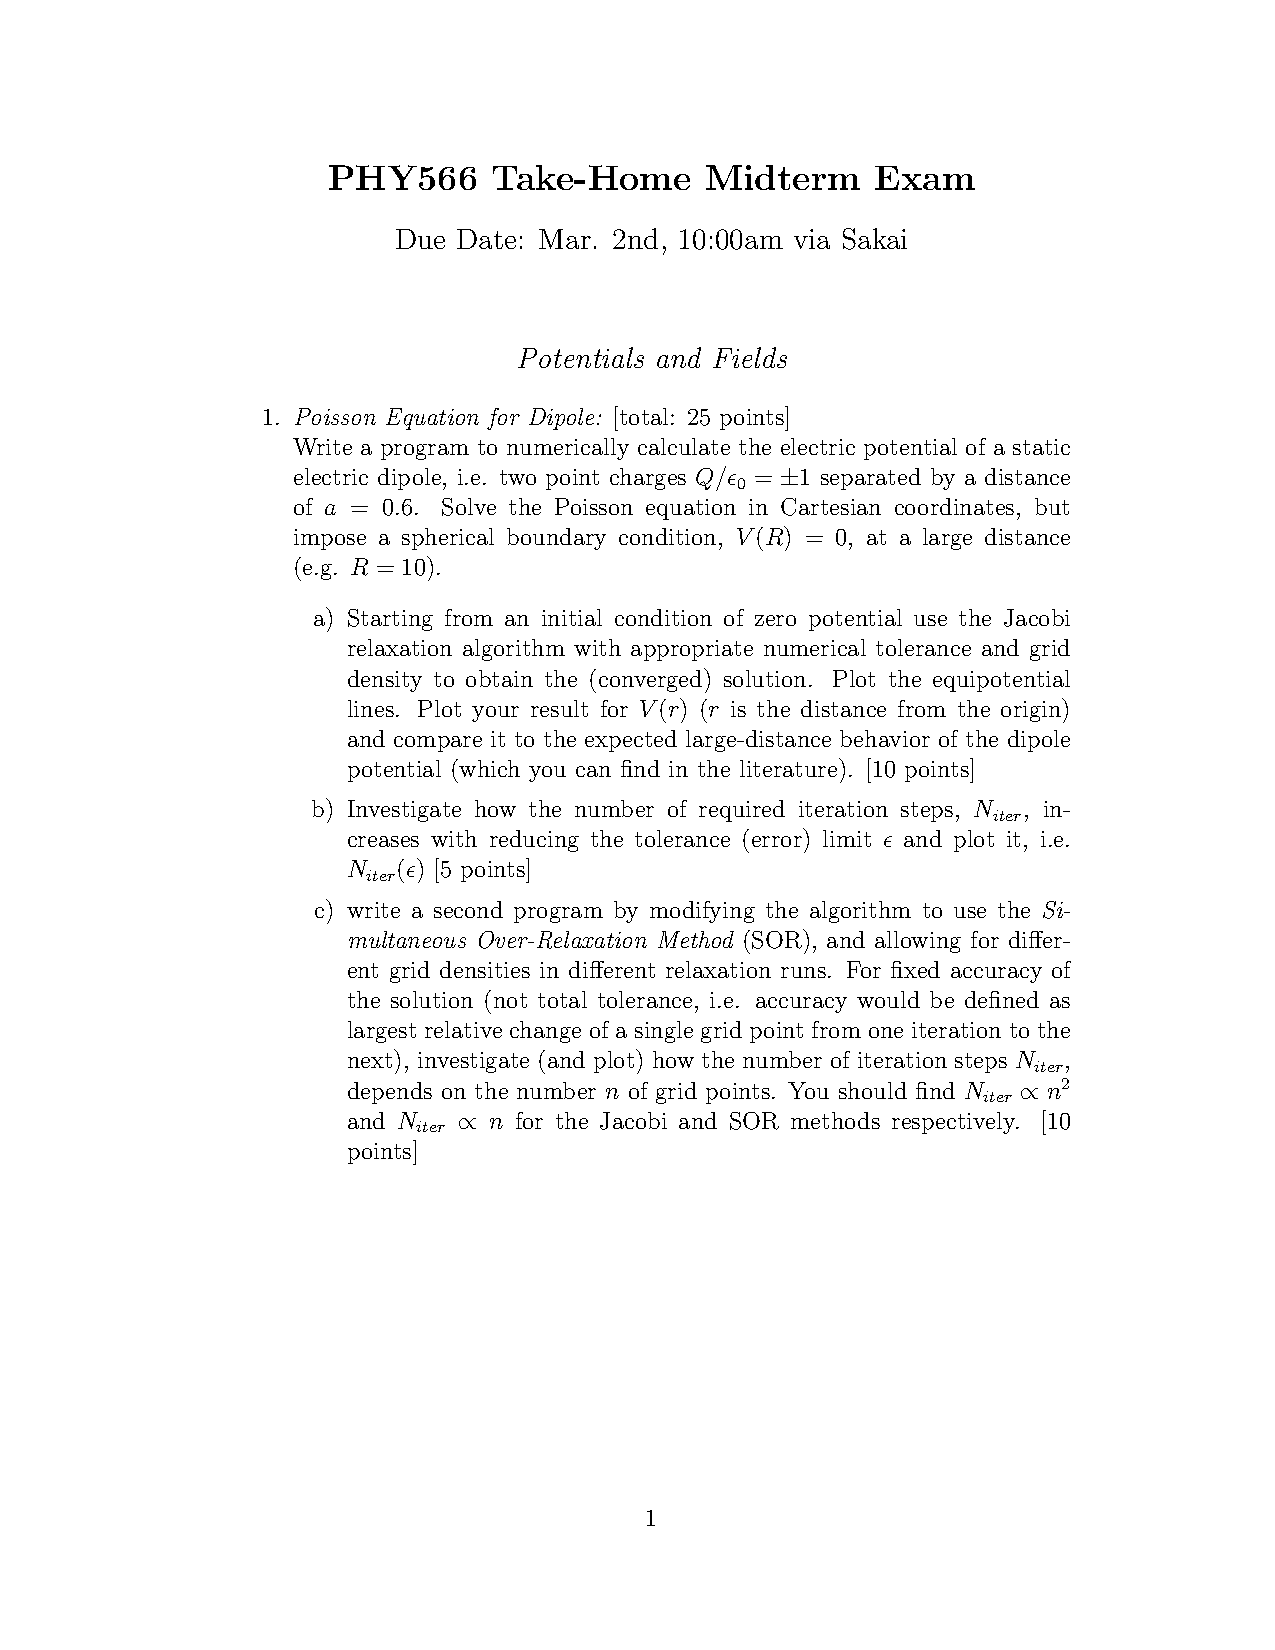
\includepdf[pages={1}]{../midterm.pdf}
\includepdf[pages={2}]{../midterm.pdf}
% Have to do them one a time for some reason or they overlap...

\clearpage
\section{Code}
\label{sec:code}

\lstinputlisting[style=python]{../code/poisson_dipole.py}
\clearpage
\lstinputlisting[style=python]{../code/biot_savart.py}

\end{document} %%% end of doc %%%
%%%%%%%%%%%%%%%%%%%%%%%%%%%%%%%%%%%%%%%%%%%%%%%%%%%%%


\bibliographystyle{bib_files/styles/atlasBibStyleWoTitle}
\bibliography{bib_files/my_bib.bib}

\begin{figure}[!htbc]
  \centering
  \includegraphics[width=.6\textwidth]{part_b/compare_runs_vary_sim_method/theta_vary_sim_method.pdf}
	{\par\nobreak\rule[9pt]{35em}{0.5pt}\vspace{-5mm}}
	\caption{$\theta\left(t\right)$ for the Euler--Cromer and RK4 methods.}
	\label{fig:theta_vary_sim_method}
\end{figure}

